%%
%% This is file `sample-sigconf.tex',
%% generated with the docstrip utility.
%%
%% The original source files were:
%%
%% samples.dtx  (with options: `all,proceedings,bibtex,sigconf')
%% 
%% IMPORTANT NOTICE:
%% 
%% For the copyright see the source file.
%% 
%% Any modified versions of this file must be renamed
%% with new filenames distinct from sample-sigconf.tex.
%% 
%% For distribution of the original source see the terms
%% for copying and modification in the file samples.dtx.
%% 
%% This generated file may be distributed as long as the
%% original source files, as listed above, are part of the
%% same distribution. (The sources need not necessarily be
%% in the same archive or directory.)
%%
%%
%% Commands for TeXCount
%TC:macro \cite [option:text,text]
%TC:macro \citep [option:text,text]
%TC:macro \citet [option:text,text]
%TC:envir table 0 1
%TC:envir table* 0 1
%TC:envir tabular [ignore] word
%TC:envir displaymath 0 word
%TC:envir math 0 word
%TC:envir comment 0 0
%%
%%
%% The first command in your LaTeX source must be the \documentclass
%% command.
%%
%% For submission and review of your manuscript please change the
%% command to \documentclass[manuscript, screen, review]{acmart}.
%%
%% When submitting camera ready or to TAPS, please change the command
%% to \documentclass[sigconf]{acmart} or whichever template is required
%% for your publication.
%%
%%
\documentclass[acmsmall,review,anonymous]{acmart}
%\documentclass[sigconf]{acmart}
%\documentclass[manuscript, screen, review, anonymous]{acmart}

\usepackage{subcaption} 


\AtBeginDocument{%
  \providecommand\BibTeX{{%
    Bib\TeX}}}

%% Rights management information.  This information is sent to you
%% when you complete the rights form.  These commands have SAMPLE
%% values in them; it is your responsibility as an author to replace
%% the commands and values with those provided to you when you
%% complete the rights form.
\setcopyright{acmlicensed}
\copyrightyear{2025}
\acmYear{2025}
\acmDOI{10.1145/XXXXXXX.XXXXXXX}




%% These commands are for a PROCEEDINGS abstract or paper.
\acmConference[SIGMOD '25]{2025 International Conference on Management of Data}{June 22--27, 2025}{Berlin, Germany}
%%
%%  Uncomment \acmBooktitle if the title of the proceedings is different
%%  from ``Proceedings of ...''!
%%
%%\acmBooktitle{Woodstock '18: ACM Symposium on Neural Gaze Detection,
%%  June 03--05, 2018, Woodstock, NY}
\acmISBN{978-1-4503-XXXX-X/25/06}

\acmSubmissionID{1505}

\begin{document}


\title[Spreadsheet Data Extractor (SDE)]{Spreadsheet Data Extractor (SDE): A Performance-Optimized, User-Centric Tool for Transforming Semi-Structured Excel Spreadsheets into Relational Data}

\author{Alexander Aue-Johr}
%\authornote{Both authors contributed equally to this research.}
\email{alexander.aue@thuenen.de}
\orcid{0009-0001-8683-3630}
\affiliation{%
  \institution{Thünen Institute for Rural Areas}
  \city{Brunswick}
  \country{Germany}
}

\author{Hardy Pundt}
%\authornote{Both authors contributed equally to this research.}
\email{hpundt@hs-harz.de}
\orcid{https://orcid.org/0000-0001-6985-5929 }
\affiliation{%
  \institution{Harz University of Applied Sciences}
  \city{Wernigerode}
  \country{Germany}
}

 

\begin{abstract}
\end{abstract}

%%
%% The code below is generated by the tool at http://dl.acm.org/ccs.cfm.
%% Please copy and paste the code instead of the example below.
%%
\begin{CCSXML}
<ccs2012>
<concept>
<concept_id>10010405.10010476.10011187.10011189</concept_id>
<concept_desc>Applied computing~Spreadsheets</concept_desc>
<concept_significance>500</concept_significance>
</concept>
<concept>
<concept_id>10002951.10002952.10003219.10003218</concept_id>
<concept_desc>Information systems~Data cleaning</concept_desc>
<concept_significance>500</concept_significance>
</concept>
<concept>
<concept_id>10011007.10011006.10011050.10010512.10003310</concept_id>
<concept_desc>Software and its engineering~Extensible Markup Language (XML)</concept_desc>
<concept_significance>500</concept_significance>
</concept>
<concept>
<concept_id>10003120.10003121.10003124.10010865</concept_id>
<concept_desc>Human-centered computing~Graphical user interfaces</concept_desc>
<concept_significance>300</concept_significance>
</concept>
<concept>
<concept_id>10003752.10003809.10010031.10002975</concept_id>
<concept_desc>Theory of computation~Data compression</concept_desc>
<concept_significance>100</concept_significance>
</concept>
</ccs2012>
\end{CCSXML}

\ccsdesc[500]{Applied computing~Spreadsheets}
\ccsdesc[500]{Information systems~Data cleaning}
\ccsdesc[500]{Software and its engineering~Extensible Markup Language (XML)}
\ccsdesc[300]{Human-centered computing~Graphical user interfaces}
\ccsdesc[100]{Theory of computation~Data compression}


\keywords{}
\begin{teaserfigure}
  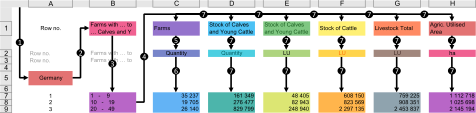
\includegraphics[width=\textwidth]{images/spreadsheet_data_extractor/livestock_hiarachy_1.pdf}
  \caption{}
  \Description{}
  \label{fig:teaser}
\end{teaserfigure}

\received{20 February 2007}
\received[revised]{12 March 2009}
\received[accepted]{5 June 2009}

\maketitle


\section{Introduction}
\cite{R}
A multitude of organizations across various sectors,
including healthcare\cite{berndt2001healthcare},
nonprofit\cite{singh2009numeric}\textsuperscript{,}
\cite{west2008because},
finance, commerce, industry, academia, and government \cite{dunn2010spreadsheets}
frequently encounter difficulties
when attempting to analyse and utilize semi-structured data derived from spreadsheets.
The absence of a defined structure within this data
presents significant challenges for analysis and utilization. 



\begin{figure*}[t]
  \centering

  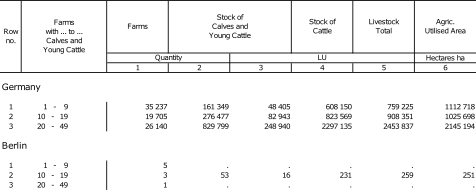
\includegraphics[width=\textwidth]{images/spreadsheet_data_extractor/livestock.pdf}

  \caption[Example data subset of the Agricultural Structure Survey on land use and livestock in Germany]{Example data subset of the Agricultural Structure Survey on land use and livestock in Germany, Source: Own figure}
  
  \label{fig:livestock}
\end{figure*}%

Nevertheless, it is not always the case that there is no structure at all.
There are cases where the data at least has "a" structure.
However, this structure is almost as helpful
as if there were simply none at all.
This is the case for data stored in spreadsheet files like Excel.
The data is not stored in a simple machine-readable wide- or long-format;
rather, it is stored in a format that is designed for human perception,
including layout with empty cells for padding, combined cells,
hierarchies in column headers, multiple tables below one another, and so on.
This is illustrated in Figure \ref{fig:livestock}
These layout techniques facilitate the comprehension of the information
by humans, but they also render the data non-machine readable.
A computer program treats the spreadsheet
as a two-dimensional array of values.
It treats empty cells in the same way
as it treats cells that contain actual data.



 


Compared to unstructured data in raw text, unstructured data in spreadsheets has the following advantages:
The hierarchy of metadata within spreadsheets is easy to comprehend for a human.
Headlines like \textit{Germany} and \textit{Berlin},
referring to our example in Figure \ref{fig:livestock},
combined column headers like \textit{Stock of Calves and Young Cattle}
on top of multiple other column headers like \textit{Quantity} and \textit{LU}
make the metadata hierarchy clear to humans.
The target data structure can be closely inspired by that visible hierarchy
and can be created with a relatively low amount of domain knowledge.
Furthermore, the values are encoded in single cells and can be uniquely
referenced by the file, sheet name and row and column index. 

The objective is to transform this data into a machine-readable form.
When considering the means to achieve this objective,
several approaches present themselves.

The SDE converts semi-structured spreadsheet data into structured formats
by allowing users to define data hierarchies without programming knowledge.

 


The Spreadsheet Data Extractor (SDE) enables users to transform the data from spreadsheets
into structured data by selecting cells containing metadata
and values to describe the data hierarchy.
To streamline the process,
users can copy previously described hierarchies to similar spaces in the sheets,
eliminating the need to select every cell and hierarchy repeatedly.  
Users do not require any programming knowledge to extract the data from the spreadsheet files.
 

Previous work by Alexander Aue, Norbert Röder, and Andrea Ackermann introduced a tool that facilitates data extraction from Excel files. While effective, this solution faced performance issues and inaccuracies in rendering cell dimensions, limiting its usability with large and complex datasets. In this paper, we build upon their foundational work by releasing the software under the open-source GNU Public License Version 3 (GPLv3) and introducing several key enhancements. These improvements include implementing incremental loading of worksheets to enhance performance, accurately rendering row heights and column widths by parsing XML data, and optimizing the rendering engine to handle large datasets efficiently. Additionally, we have integrated the selection hierarchy and worksheet view into a unified interface to improve user experience. These contributions collectively address the limitations of the existing solution, making data extraction from complex spreadsheets more efficient and user-friendly.
 
\section{Contribution}

Wir bauen auf der bestehenden Arbeit von Alexander Auer, Norbert Röder und Andrea Ackermann auf. Zusätzlich dazu veröffentlichen wir die Software nun unter der Open Source Lizenz GNU Public Licence Version 3 und tragen folgende Verbesserungen bei. Die bestehende Lösung nutzte das Dart-Package excel, um die .xlsx-Dateien zu öffnen. Dies war jedoch sehr langsam, da das Paket die gesamte .xlsx-Datei zunächst vollständig einliest. Wir haben daher eine eigene Funktionalität in Dart implementiert, die die Excel-Arbeitsblätter inkrementell lädt.
Außerdem hat die bestehende Lösung die Zellwerte aus der .xlsx-Datei ausgelesen, dabei jedoch die Breiten und Höhen der Zeilen und Spalten ignoriert und stattdessen deren Größe selbst berechnet, basierend auf dem in den Zellen enthaltenen Text. Dies führte jedoch zu sehr breiten Zellen, die in der ursprünglichen Datei tatsächlich deutlich schmaler waren. Dies lag daran, dass einige Zellen in derselben Spalte sehr langen Text enthielten, um einen Titel darin zu speichern. Durch diese übermäßig breiten Spalten wurde die Navigation durch das Arbeitsblatt erschwert.
Im Vergleich zur ursprünglichen Lösung bietet unsere Version eine Funktionalität, die die Spalten- und Zeilenhöhen und -breiten korrekt ausliest und diese so darstellt, wie es Excel tut. So wird der Benutzer nicht von der Darstellung überrascht.
Die bestehende Lösung hat weiterhin die Zellen gezeichnet, selbst wenn sie nicht im.Aktuellen Viewport sichtbar waren. Das Städte erhebliche Probleme da, wenn Arbeitsblätter mit sehr vielen Zellinhalten geöffnet worden. Die Performance Sankt dabei so stark herab, dass das Programm nicht mehr benutzbar war.Aus diesem Grund haben wir einen Mechanismus implementiert, dass nur zellinhalte gezeichnet werden, die auch tatsächlich sichtbar sind.


\begin{table*}[h]
  \centering
  \begin{tabular}{|c|c|c|c|c|}
      \hline
      \textbf{Name} & \textbf{Technologies} & \textbf{Output} & \textbf{Accessibility} & \textbf{Frequency} \\ \hline
      DeExcelerator & heuristics            & cleaned data    & partially open source  & last publication   \\
                    &                       &                 &                & 2015               \\ \hline
      FlashRelate   & AI               & cleaned data    & proprietary,           & last publication   \\
                    & programming-by-example &                 & no access              & 2015               \\ \hline


      Senbazuru     & AI               & cleaned data    & partially open source  & last commit        \\
                    &                       &                 &                        & 2015               \\\hline

      XLindy        & AI                    & cleaned data    & no access              & cancelled          \\ \hline
      TableSense    & AI                    & diagrams        & proprietary,           & last commit        \\
                    &                       &                 & no access              & 2021               \\ \hline
  \end{tabular}
  \caption{Spreadsheet Data Extractor counterparts}

  \label{tab:approaches}
\end{table*}
\section{Related Work}

The extraction of relational data from semi-structured documents, particularly spreadsheets, has garnered significant attention due to their ubiquitous use across domains such as business, government, and scientific research. Several frameworks and tools have been developed to address the challenges of converting flexible spreadsheet formats into normalized relational forms suitable for data analysis and integration. Notable among these are \textbf{DeExcelerator}, \textbf{XLIndy}, \textbf{FLASHRELATE}, \textbf{Senbazuru}, \textbf{TableSense} und den Ansatz von Aue et al. auf dessen arbeit wir aufbauen.

\subsection{Aue et al.'s Converter}

Aue et al.~\cite{alexander2024converting} developed a tool aimed at facilitating data extraction from Excel spreadsheets by utilizing the Dart `excel` package to open `.xlsx` files. Users can select cells containing data and metadata to define the data hierarchy. However, this method encounters performance bottlenecks as the package requires loading the entire `.xlsx` file into memory before processing, leading to slow response times, especially with large files. Additionally, their solution calculates row heights and column widths based solely on cell content, disregarding the actual dimensions specified in the Excel file. This results in discrepancies between the tool's rendering and the original spreadsheet. The tool also renders all cells regardless of their visibility within the viewport, causing significant performance degradation when handling worksheets with numerous cells.

\subsection{DeExcelerator}

Eberius et al.~\cite{eberius2013deexcelerator} introduced \textbf{DeExcelerator}, a framework that transforms partially structured spreadsheets into first normal form relational tables using heuristic-based extraction phases. It addresses challenges such as table detection, metadata extraction, and layout normalization. While effective in automating normalization, its reliance on predefined heuristics limits adaptability to heterogeneous or unconventional spreadsheet formats, highlighting the need for more flexible approaches.

\subsection{XLIndy}

Koci et al.~\cite{koci2019xlindy} developed \textbf{XLIndy}, an interactive Excel add-in with a Python-based machine learning backend. Unlike DeExcelerator’s fully automated heuristic approach, XLIndy integrates machine learning techniques for layout inference and table recognition, enabling a more adaptable and accurate extraction process. XLIndy's interactive interface allows users to visually inspect extraction results, adjust configurations, and compare different extraction runs, facilitating iterative fine-tuning. Additionally, users can manually revise predicted layouts and tables, saving these revisions as annotations to improve classifier performance through (re-)training. This user-centric approach enhances the tool’s flexibility, allowing it to accommodate diverse spreadsheet formats and user-specific requirements more effectively than purely heuristic-based systems.

\subsection{FLASHRELATE}

Barowy et al.~\cite{barowy2015flashrelate} presented \textbf{FLASHRELATE}, an approach that empowers users to extract structured relational data from semi-structured spreadsheets without requiring programming expertise. FLASHRELATE introduces a domain-specific language, \textbf{FLARE}, which extends traditional regular expressions with spatial constraints to capture the geometric relationships inherent in spreadsheet layouts. Additionally, FLASHRELATE employs an algorithm that synthesizes FLARE programs from a small number of user-provided positive and negative examples, significantly simplifying the automated data extraction process.

FLASHRELATE distinguishes itself from both DeExcelerator and XLIndy by leveraging programming-by-example (PBE) techniques. While DeExcelerator relies on predefined heuristic rules and XLIndy incorporates machine learning models requiring user interaction for fine-tuning, FLASHRELATE allows non-expert users to define extraction patterns through intuitive examples. This approach lowers the barrier to entry for extracting relational data from complex spreadsheet encodings, making the tool accessible to a broader range of users.

\subsection{Senbazuru}

Chen et al.~\cite{chen2013senbazuru} introduced \textbf{Senbazuru}, a prototype Spreadsheet Database Management System (SSDBMS) designed to extract relational information from a large corpus of spreadsheets. Senbazuru addresses the critical issue of integrating data across multiple spreadsheets, which often lack explicit relational metadata, thereby hindering the use of traditional relational tools for data integration and analysis.

Senbazuru comprises three primary functional components:

\begin{enumerate}
    \item \textbf{Search}: Utilizing a textual search-and-rank interface, Senbazuru enables users to quickly locate relevant spreadsheets within a vast corpus. The search component indexes spreadsheets using Apache Lucene, allowing for efficient retrieval based on relevance to user queries.
    
    \item \textbf{Extract}: The extraction pipeline in Senbazuru consists of several stages:
    \begin{itemize}
        \item \textbf{Frame Finder}: Identifies data frame structures within spreadsheets using Conditional Random Fields (CRFs) to assign semantic labels to non-empty rows, effectively detecting rectangular value regions and associated attribute regions.
        \item \textbf{Hierarchy Extractor}: Recovers attribute hierarchies for both left and top attribute regions. This stage also incorporates a user-interactive repair interface, allowing users to manually correct extraction errors, which the system then generalizes to similar instances using probabilistic methods.
        \item \textbf{Tuple Builder and Relation Constructor}: Generates relational tuples from the extracted data frames and assembles these tuples into coherent relational tables by clustering attributes and recovering column labels using external schema repositories like Freebase and YAGO.
    \end{itemize}
    
    \item \textbf{Query}: Supports basic relational operations such as selection and join on the extracted relational tables, enabling users to perform complex data analysis tasks without needing to write SQL queries.
\end{enumerate}

Senbazuru's ability to handle hierarchical spreadsheets, where attributes may span multiple rows or columns without explicit labeling, sets it apart from earlier systems like DeExcelerator and XLIndy. By employing machine learning techniques and providing user-friendly repair interfaces, Senbazuru ensures high-quality extraction and facilitates the integration of spreadsheet data into relational databases.


\subsection{TableSense}

Dong et al.~\cite{dong2019tablesense} developed \textbf{TableSense}, an end-to-end framework for spreadsheet table detection using Convolutional Neural Networks (CNNs). TableSense addresses the diversity of table structures and layouts by introducing a comprehensive cell featurization scheme, a Precise Bounding Box Regression (PBR) module for accurate boundary detection, and an active learning framework to efficiently build a robust training dataset.

While \textbf{DeExcelerator}, \textbf{XLIndy}, \textbf{FLASHRELATE}, and \textbf{Senbazuru} focus primarily on transforming spreadsheet data into relational forms through heuristic, machine learning, and programming-by-example approaches, \textbf{TableSense} specifically targets the accurate detection of table boundaries within spreadsheets using deep learning techniques. Unlike region-growth-based methods employed in commodity spreadsheet tools, which often fail on complex table layouts, TableSense achieves superior precision and recall by leveraging CNNs tailored for the unique characteristics of spreadsheet data.
However, TableSense focuses on table detection and visualization, allowing users to generate diagrams from the detected tables but does not provide functionality for exporting the extracted data for further analysis.


\subsection{Comparison and Positioning}

While \textbf{DeExcelerator}, \textbf{XLIndy}, \textbf{FLASHRELATE}, \textbf{Senbazuru}, and \textbf{TableSense} each offer unique approaches to spreadsheet data extraction, they share certain limitations. Many of these tools are not readily accessible: \textbf{FLASHRELATE} and \textbf{TableSense} are proprietary, and \textbf{Senbazuru}, \textbf{XLIndy}, and \textbf{DeExcelerator} are discontinued projects with limited or no source code availability. In contrast, we contribute our spreadsheet data extractor under the GNU General Public License v3.0, allowing the community to access, use, and improve the tool freely.

Moreover, unlike the aforementioned tools that rely on heuristics, machine learning, or AI techniques—which can introduce errors requiring users to identify and correct—we adopt a user-centric approach that gives users full control over data selection and metadata hierarchy definition. While this requires more manual input, it eliminates the uncertainty and potential inaccuracies associated with automated methods. To streamline the process and enhance efficiency, our tool includes user-friendly features such as the ability to duplicate hierarchies of columns and tables, and to move them over similar structures for reuse, reducing the need for repetitive configurations.



By combining the strengths of manual control with enhanced user interface features and performance optimizations, our tool offers a robust and accessible solution for extracting relational data from complex and visually intricate spreadsheets. These enhancements not only improve performance and accuracy but also elevate the overall user experience, making our tool a valuable asset for efficient and reliable data extraction from diverse spreadsheet formats.

 





\section{Methodology}


In Abbildung 
\ref{fig:nothing} ist die Ansicht des Spreadsheet Data extractor tu sehen. Oben links zeught die Liste der Zell selektionen die aktuell noch leer ist. Oben rechts ist die ansicht des aktuell geäffneten Excel Worksheets und unten wird die ausgabe der zell Selektion angezeigt um sofortiges feedback zu erhalten, ob die vorgenommenen Selektionen die gewünschte ausgabe liefern.

\begin{figure}[h]
  \centering
  \includegraphics[width=\textwidth]{images/spreadsheet_data_extractor/new_version/nothing.png}
  \caption{}
  \label{fig:nothing}
\end{figure}%

Abbildung \ref{fig:first_column} zeigt die Selektion der ersten Spalte. Dazu wurde ein knoten eingefügt und anschließend auf die Metainformation geklickt, welche die meisten Zellen in dem Arbeitsblatt gemeinsam haben und die dementsprechend in der csv Datei am Anfang auftauchen sollte. In diesem Fall ist dies die Zelle mit dem Wert "Nursing Staff". In jedem Knoten können weitere Knoten eingebettet werden, die als eingerückte  Kinder des aktuellen Knotens darstellt werden. Das nächste Kind ist die Zelle  "Total", denn sie beschreibt die erste Untertabelle. Gleichzeitig ist diese Zelle nicht nur Überschrift für die Tabelle sondern beschreibt gleichzeitig die Zeile für die Summe der Pflegekräfte. Deshalbt taucht "Total" auch in der nächsten Selektion auf, in der alle Zeilenbeschriftungen stehen: "Total", "15-20", "20-25".

Als nächstes kann die Erste Spalte mit Daten eingefügt werden, dafür wird der nächste eingegebbete Knoten der Spaltenheader "2024" und der nächste Knoten ist wieder eine liste, dieses mal die Zellwerte der ersten Spalte.


\begin{figure}[h]
  \centering
  \includegraphics[width=\textwidth]{images/spreadsheet_data_extractor/new_version/first_column.png}
  \caption{}
  \label{fig:first_column}
\end{figure}%

Die nächsten5 Spalten müssen nicht genau so manuell eingetragen werden, die die erste, denn die Hiearchie der ersten spalte kann einfach kopiert und auf die anderen Spalten angewendet werden. Dazu wird der Knoten der  ersten Spalte "2024" selektiert und darauf rechtsgegklickt. Ein Popup öffnet sich in dem die Aktion "move and duplicate" auftaucht, die nun geklickt werden sollte, wie in Abbildung \ref{fig:move_and_duplicate_2024} zu sehen ist.

\begin{figure}[h]
  \centering
  \includegraphics[width=\textwidth]{images/spreadsheet_data_extractor/new_version/move_and_duplicate_2024.png}
  \caption{}
  \label{fig:move_and_duplicate_2024}
\end{figure}%


Daraufhin öffnet sich in der App bar oben im Bild eine reiche von schaltflächen ,duie erlauben die Zellenselektionen des knotens sowie aller Kinderknoten zu verschieben wie in Abbildung \ref{fig:5_repetitions} zu sehen ist. Durch das drücken auf die Schaltfläche zum verschieben der Selektion um eine einheit nach rechts ist bereits die nächste Spalte 2029 fertig aselektiert. Auf die gleich Art und weise können nun auch die nächsten Spalten selektiert werden. doch das geht auch schneller, denn statt nur einmal die selektion zu verschieben und gleichzeitig zu stornierenn, kann auch das eingabefeld "repeat" mit so vielen Wiederholungen gefüllt werden, wie es Spalten gibt. Mit der Eingabe der Nummer 5 sind damit alle Spalten ausgewählt.

\begin{figure}[h]
  \centering
  \includegraphics[width=\textwidth]{images/spreadsheet_data_extractor/new_version/5_repetitions.png}
  \caption{}
  \label{fig:5_repetitions}
\end{figure}%


Das gleiche was für die Spalten bereits so gut funktioniert hat, kann nun auch für die Untertabellen wiederholt werden, wie in Abbildung \ref{fig:all_cells_selected} zu sehen ist.

Durch das Selektieren des Knotens mit dem Wert "Total" und das drücken auf die Schaltfläche "move and duplicate" kann die Selektion der Untertabelle "Total" auf die anderen Untertabellen angewendet werden. Dazu muss die Tabelle um so viele Zeilen nach unten verschoben werden, bis sie mit der untertabelle überlappt  Dabei gibt es nur ein kleines Problem. Denn zu den Unterknoten des Knotens "Total" gehören auch die Spaltenheader dazu. Würden diese Spaltenheader in der Untertabelle darunter wiederholt werden, würde das verschieben der Selektionen nach unten unverändert funktionieren. Doch dadurch, dass diese Zellen in den untertabellen nicht wiederholt werden, , muss dafür gesorgt werden, dass sich die Zellen mit den Spaltenheadern daran gehindert werden sich durch die funkion zum verschieben und kopieren mit verschoben werden. Zu diesem Zweck können einzelne Knoten von der verschiebung ausgenommen werden, dazu muss lediglich das Vorhägeschlock button geklickt werden, wodurch die Zellselektion nicht mehr in der verschiebung enthalten ist. Sie bleibt starr an ihrem ursprungsort, egal ob die anderen Zellen verschoben werden. Desshalb werden nun die Knoten mit den SPaltenheadern, also die mit  den Jahreszahlen 2024 bis 2049 identifiziert und selektiert und über den button mit dem Vorhängeschloss die Zellselektion die starr bleibt. Durch das verschieben nach unten und durch das damit verbundene duplizieren können nun sehr einfach die Zellselektionen nach unten verschoben und dupliziert werden. Durch das einsellen von 2 Wiederholungen werden alle untertabellen komplett ausgewählt.
 {fig:all_cells_selected} zu sehen ist.

\begin{figure}[h]
  \centering
  \includegraphics[width=\textwidth]{images/spreadsheet_data_extractor/new_version/all_cells_selected.png}
  \caption{}
  \label{fig:all_cells_selected}
\end{figure}%

This section outlines the technical foundation and software architecture of our enhanced tool. We detail the methods employed to achieve a realistic representation of Excel files, optimize performance when handling large datasets, and integrate an intuitive user interface that streamlines the data extraction process.

Die ausgabe wird wir folgt berechnet. Das ist in Abbildung \ref{fig:hierachy} anhand der ersten drei spalten sowie der ersten drei Zellen der Tabelle die wir als zu demonstrationsgründen so vereinfach haben. 
 
\begin{figure}[h]
  \centering
  \includegraphics[width=\textwidth]{images/spreadsheet_data_extractor/new_version/hierachy.pdf}
  \caption{}
  \label{fig:hierachy}
\end{figure}%

AUf diese  hiearachie wird cross product angewendet was die hiarachy in eine datenstruktur umwandelt wie sie in Abbildung x zu sehen ist. Alle Einträge, die genau eine Zeile haben werden so häfig durch duplizieren in ihrer anzahlerhöhnt , bis die Anzahl der Anzahl des letzten Knotens gleicht. Ist die Selektion allerdings eine Liste von Zellen, so wird an ihr nichts verändert.

\begin{figure}[h]
  \centering
  \includegraphics[width=\textwidth]{images/spreadsheet_data_extractor/new_version/hierachy_cross_product.pdf}
  \caption{}
  \label{fig:hierachy}
\end{figure}%

\subsection{Software Architecture Overview}

The tool is developed using the Flutter Software Development Kit (SDK), a cross-platform UI toolkit that allows for high-performance applications on various operating systems. Flutter provides a flexible and efficient framework for building complex user interfaces with smooth animations and responsiveness, which is essential for our application's requirements.

The architecture consists of three main layers:

\begin{enumerate}
    \item \textbf{Data Parsing Layer}: Responsible for reading and interpreting Excel files, extracting cell data, styles, and structural information.
    \item \textbf{Rendering Layer}: Handles the visual representation of the spreadsheet, including cell dimensions, styles, and layouts.
    \item \textbf{User Interface Layer}: Provides interactive components for users to select data, define hierarchies, and manage the extraction process.
\end{enumerate}

These layers interact seamlessly to provide a cohesive user experience, enabling users to work with large and complex spreadsheets efficiently.

\subsection{Data Parsing and Representation}

\subsubsection{Excel File Parsing}

To accurately replicate the structure and appearance of Excel files, the tool parses the underlying XML content of the \texttt{.xlsx} format, which is essentially a collection of XML files packaged in a ZIP archive. We utilize libraries compatible with Flutter to handle ZIP extraction and XML parsing.

Key steps in the parsing process include:

\begin{itemize}
    \item \textbf{Workbook and Worksheet Identification}: Extracting the list of worksheets and their relationships from the \texttt{workbook.xml} file.
    \item \textbf{Cell Data Extraction}: Parsing individual \texttt{sheetN.xml} files to read cell values, types, and references.
    \item \textbf{Shared Strings Handling}: Accessing the \texttt{sharedStrings.xml} file to retrieve string values that are referenced by index in the cell data.
    \item \textbf{Styles and Formatting}: Parsing the \texttt{styles.xml} file to extract information about cell styles, including fonts, fills, borders, and number formats.
\end{itemize}

\subsubsection{Calculating Cell Dimensions}

Excel stores cell dimensions in units that do not directly correspond to pixels. To render cells accurately, we calculate the pixel dimensions using the following methods:

\begin{itemize}
    \item \textbf{Column Widths}: Extracted from the \texttt{<col>} elements in the worksheet XML, representing the width in units based on the average character width. We apply a scaling factor of \textbf{7} to convert these units to pixels. This factor was determined empirically to match the on-screen appearance of Excel columns.
    \item \textbf{Row Heights}: Specified in points (1/72 of an inch) within the \texttt{<row>} elements. We multiply the height values by \textbf{4/3} to convert points to pixels, aligning with the standard screen resolution of 96 DPI (dots per inch).
\end{itemize}

These scaling factors ensure that the rendered spreadsheet in our tool mirrors the dimensions users expect from Excel, facilitating accurate data selection.

\subsubsection{Rendering Cell Styles}

We enhance the visual fidelity by applying cell styles during rendering:

\begin{itemize}
    \item \textbf{Background Colors}: Extracted from the \texttt{<fill>} elements in \texttt{styles.xml}, we map the style indices from the cell data to the corresponding color definitions. Colors are processed in ARGB format for accurate display.
    \item \textbf{Borders}: We parse border definitions to render cell edges appropriately. This includes the style (e.g., solid, dashed) and color of each border side.
    \item \textbf{Merged Cells Handling}: Merged cells are identified through the \texttt{<mergeCells>} elements. We account for merged regions by appropriately adjusting the rendering of cell spans.
\end{itemize}

\subsection{Rendering Engine}

The rendering engine leverages Flutter's high-performance graphics capabilities to display the spreadsheet efficiently.

\subsubsection{Viewport-Based Rendering}

To manage performance with large spreadsheets, we implement a viewport-based rendering approach:

\begin{itemize}
    \item \textbf{Visible Area Calculation}: Determine the range of rows and columns currently visible in the user's viewport based on scroll position and zoom level.
    \item \textbf{On-Demand Rendering}: Only the cells within the visible area are rendered. As the user scrolls, new cells entering the viewport are rendered, while those exiting are discarded.
    \item \textbf{Smooth Scrolling and Zooming}: Flutter's rendering pipeline ensures that scrolling and zooming operations are smooth, even with dynamic loading of cell content.
\end{itemize}

\subsubsection{Asynchronous Data Loading}

We employ asynchronous operations to prevent blocking the user interface:

\begin{itemize}
    \item \textbf{Background Parsing}: Cell data and styles are loaded in the background, allowing the UI to remain responsive.
    \item \textbf{Progress Indicators}: Visual feedback is provided to inform users of loading states, especially when accessing new worksheets or large data ranges.
\end{itemize}

\subsection{User Interface Design}

\subsubsection{Integrated Selection and Hierarchy Management}

We redesigned the user interface to integrate the selection hierarchy with the worksheet view:

\begin{itemize}
    \item \textbf{Unified Workspace}: Users can select cells and manage the data hierarchy within the same view, eliminating the need to switch contexts.
    \item \textbf{Interactive Hierarchy Panel}: A sidebar displays the hierarchical structure of selections, allowing users to drag and drop elements to adjust relationships.
    \item \textbf{Contextual Actions}: Right-click menus and toolbars provide quick access to common actions such as duplicating selections, setting parent-child relationships, and adjusting properties.
\end{itemize}

\subsubsection{Selection Tools and Shortcuts}

To facilitate efficient data selection, we introduced advanced selection tools:

\begin{itemize}
    \item \textbf{Range Selection}: Users can select multiple cells by clicking and dragging or by entering cell references manually.
    \item \textbf{Duplication and Movement}: Selections can be duplicated and moved across the worksheet. Users specify the number of duplicates and the direction of movement, streamlining the process of selecting repetitive data structures.
    \item \textbf{Freezing Elements}: Certain selections can be `frozen` during duplication, maintaining their position while other elements are moved. This is useful for headers or labels that remain constant.
\end{itemize}

\subsection{Performance Optimization Strategies}

\subsubsection{Incremental Worksheet Loading}

To reduce initial load times:

\begin{itemize}
    \item \textbf{Lazy Loading of Worksheets}: Worksheets are parsed only when the user selects them. This defers unnecessary processing and conserves resources.
    \item \textbf{Resource Management}: Unused worksheets are unloaded from memory after a period of inactivity, preventing excessive memory consumption.
\end{itemize}

\subsubsection{Efficient Data Structures}

We optimize data handling through:

\begin{itemize}
    \item \textbf{Sparse Data Representation}: Only non-empty cells are stored in memory, utilizing maps or hash tables keyed by cell references.
    \item \textbf{Indexing Mechanisms}: Indexes are built for quick access to cell data and styles, reducing lookup times during rendering and interaction.
\end{itemize}

\subsubsection{Caching and Reuse}

\begin{itemize}
    \item \textbf{Render Cache}: Recently rendered cells are cached to minimize redraws when scrolling back and forth.
    \item \textbf{Data Cache}: Frequently accessed data, such as styles and shared strings, are cached for quick retrieval.
\end{itemize}

\subsection{Data Extraction Process}

The extraction process translates user selections into a structured data format:

\begin{itemize}
    \item \textbf{Hierarchy Flattening}: The tool traverses the selection hierarchy, combining metadata and data selections to construct records.
    \item \textbf{Relation Mapping}: Parent-child relationships define how data fields relate, enabling the creation of relational tables.
    \item \textbf{Data Transformation}: Cell values are extracted, and any necessary transformations (e.g., data type conversions, trimming whitespace) are applied.
\end{itemize}

\subsubsection{Export Formats}

The tool supports exporting data in various formats:

\begin{itemize}
    \item \textbf{CSV Files}: Standard comma-separated values for compatibility with most data analysis software.
    \item \textbf{JSON}: For applications requiring structured data with nested objects.
    \item \textbf{Database Import}: Direct import into databases through connectors or by generating SQL scripts.
\end{itemize}

\subsection{Validation and Error Handling}

To ensure data integrity:

\begin{itemize}
    \item \textbf{Input Validation}: The tool checks for invalid selections, such as overlapping ranges or circular hierarchies, and prompts users to correct them.
    \item \textbf{Error Reporting}: Any issues encountered during parsing or exporting are reported with detailed messages to assist in troubleshooting.
    \item \textbf{Undo/Redo Functionality}: Users can revert actions, encouraging experimentation without the risk of losing progress.
\end{itemize}

\subsection{Summary of Methodology}

Our methodology focuses on combining technical innovations with user-centric design principles. By parsing Excel files at a granular level and accurately rendering their visual aspects, we enable users to interact with spreadsheets naturally. Performance optimizations ensure that the tool remains responsive, even with large datasets. The integrated user interface simplifies the data extraction process, making it accessible to users without programming expertise.



\section{Methodology}

\begin{figure*}[h]
  \begin{subfigure}{1.0\textwidth}
    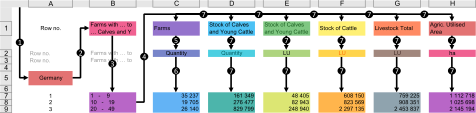
\includegraphics[width=\textwidth]{images/spreadsheet_data_extractor/livestock_hiarachy_1.pdf}
    \caption{The data selection view, once all selections are completed}
    \label{fig:livestock_hiarachy_1}
  \end{subfigure}
  \begin{subfigure}{1.0\textwidth}
    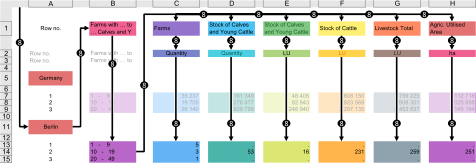
\includegraphics[width=\textwidth]{images/spreadsheet_data_extractor/livestock_hiarachy_2.pdf}
    \caption{The data selection view, once all selections are completed}
    \label{fig:livestock_hiarachy_2}
  \end{subfigure}
  \caption[Second Level Third Level Questions]{Second Level Third Level Questions, Source: Own figure}
  \label{fig:livestock_hiarachy}  
\end{figure*}

We used the software development kit Flutter
to develop a program with a user interface
that allows the selection of the cells containing the metadata
and data inside the spreadsheet.
We refer again to the example from Figure \ref{fig:livestock}
to describe the necessary steps
required for data extraction from spreadsheets.
We use this example spreadsheet to illustrate
the necessary steps required for data extraction
from spreadsheets like this one.
When looking at the spreadsheet,
a human can identify a hierarchy very easily.
There are sub-tables with headings,
and all the sub-tables share the same columns,
which are only laid out once at the top of the spreadsheet
rather than being repeated for each sub-table.

The headings \textit{Germany} and \textit{Berlin} in this example
are the topmost metadata because most cells containing actual data
share these headings as common metadata,
whereas the metadata of the column header \textit{Agric. Utilised Area}
and \textit{Hectares ha} is only shared by the cells beneath that column.
A human can see these hierarchies,
but to a program, these hierarchies are not visible;
the program just sees a two-dimensional grid of cells,
some empty, some containing text, and some containing numbers.

The computer needs to be able to interpret this hierarchy in the spreadsheet
just as a human does.
However, for that to happen, it needs the hierarchy as input.
Our approach is that the user provides this hierarchy
to the computer by selecting the cells and describing the relationships
they have to one another.

To make this process easier and faster for the user,
the amount of user interaction should be minimized as much as possible.
This can be achieved by selecting the most abstract meta-information first
and then progressively narrowing down to increasingly specific meta-information
until the actual facts are chosen.
Additionally, allowing the user to duplicate selections and hierarchies
to similar areas in the spreadsheet can streamline this process.






\begin{figure*}[!t]
  \centering
  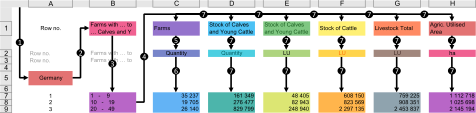
\includegraphics[width=\textwidth]{images/spreadsheet_data_extractor/livestock_hiarachy_1.pdf}
  \caption{The data selection view, once all selections are completed}
  \label{fig:livestock_hiarachy_1}
\end{figure*}




 
In Figure \ref{fig:livestock_hiarachy_1}, cells are presented
as they appear within our program's data selection view
after all the selections are made.
Additionally, an additional layer with black arrows illustrates
the optimal sequence of selections for this example,
designed to minimize user interaction.
These arrows, numbered from 1 to 7, represent the specific steps of user interaction.








Please note that the program deconstructs merged cells.
Cells from which the merged cell was created are displayed as individual cells (e.g. \textit{Quantity} and \textit{LU}).
This will be useful for the following selections.


\begin{figure}[h]
    \centering
 
    \includegraphics[width=0.5\textwidth]{images/spreadsheet_data_extractor/duplicate_and_move.png}
 
    \caption[Selecting the tables arranged one below the other]{Selecting the tables arranged one below the other}
    
    \label{fig:duplicate_and_move}
\end{figure}%

The most abstract meta-information, which is the meta-information shared by most cells, is the country or state in this example (Arrow 1). After that, the header of the domain of the relation is selected (Arrow 2) and then the domain itself will be picked (Arrow 3). While Selections 1 and 2 each selected individual cells, Selection 3 introduces the concept of choosing a set of cells.
Moving on to the first data column, the process involves selecting the first column header (Arrow 4), followed by choosing the second column header (Arrow 5). Now, the first range of the relation is selected (Arrow 6).
If the selection of data were to continue in the same manner, this would involve an additional 15 selections just for the first table, offering no significant improvement over manually creating the relation by simply copying and pasting the cells. However, the subsequent selections can be automated,
given that both two column headers and the numeric values are located in the same row, each one cell to the right of the previous one. The program's \textit{Duplicate and Move} function allows these cells to be selected in a single step.
To do this, Selection 4 is chosen, and the duplicate is moved one cell to the right.

A slider can be adjusted to determine the number of duplicates to generate. Each duplicate is moved the same number of cells in the same direction as the previous one.
For this example, the slider is set to create 5 duplicates (see Figure \ref{fig:duplicate_and_move}).
This results in all the selections depicted as arrows labelled 7 in Figure \ref{fig:livestock_hiarachy_1}.

This functionality is made possible by the Spreadsheet Data Extractor's ability
to deconstruct merged cells, such as those in the \textit{Quantity} and \textit{LU} columns.
Without this feature, duplicating and moving selections over these merged columns would fail,
resulting in the cells within the \textit{Quantity} and \textit{LU} columns remaining empty, except for the first cell in each merged group.
However, the Spreadsheet Data Extractor displays the underlying cells of the merged cells as redundant copies.
This approach allows the process of duplicating and moving column selections over these merged areas to work seamlessly.
With this, the first table is captured.



The same procedure used to capture the previous five columns
can be applied to capture the tables arranged below one another.
To do this, Selection 1 is chosen, then duplicated and moved down by six cells.
However, the header cells (B1 to H2) are an exception to this,
because they don't reappear in the tables below.
The program offers a freeze option for this purpose.
The frozen cells are duplicated but remain in their original positions during the move.
Figure \ref{fig:livestock_hiarachy_2} illustrates how the \textit{Duplicate and Move} function was employed
to capture the table below by moving all but the frozen cells down
by six cells (all arrows labelled with the number 8).


After the selections are made,
the hierarchy of selections forms a tree
in which each node contains the selected set of cells.
Except for the first two nodes,
where the first node represents the spreadsheet file (e.g. \textit{Livestock.xlsx})
and the second node represents the workbook's worksheet (e.g. \textit{Calves}). 
This is demonstrated in Figure \ref{fig:tree_horizontal_small}
for the subtree with the root node \textit{Germany}.


\begin{figure*}[ht]
  \begin{subfigure}{1.0\textwidth}
    \includegraphics[width=\textwidth]{images/spreadsheet_data_extractor/tree_horizontal_small_v2.pdf}
    \caption[Tree structure of cell sets of subtree Germany]{Tree structure of cell sets of subtree Germany, Source: Own figure}
    \label{fig:tree_horizontal_small}
  \end{subfigure}
  \begin{subfigure}{1.0\textwidth}
    \includegraphics[width=\textwidth]{images/spreadsheet_data_extractor/tree_product_horizontal_small_v2.pdf}
    \caption[Cross Product of subtree Germany]{Cross Product of subtree Germany, Source: Own figure}
    \label{fig:tree_product_horizontal_small}
  \end{subfigure}
  \caption[Second Level Third Level Questions]{Second Level Third Level Questions, Source: Own figure}
  \label{fig:livestock_hiarachy}  
\end{figure*}



\begin{figure*}[t]
    \centering
    \includegraphics[width=\textwidth]{images/spreadsheet_data_extractor/tree_horizontal_small_v2.pdf}
    \caption[Tree structure of cell sets of subtree Germany]{Tree structure of cell sets of subtree Germany, Source: Own figure}
    \label{fig:tree_horizontal_small}
\end{figure*}%


\begin{figure*}[t]
  \centering
  \includegraphics[width=\textwidth]{images/spreadsheet_data_extractor/tree_product_horizontal_small_v2.pdf}
  \caption[Cross Product of subtree Germany]{Cross Product of subtree Germany, Source: Own figure}
  \label{fig:tree_product_horizontal_small}
\end{figure*}%


To transform this tree of sets of cells into relational data,
we calculate the cross product of the tree.
The length of each child set is obtained from the bottom up,
and the parent node is duplicated as many times as necessary
to match the length of that child set (Figure \ref{fig:tree_product_horizontal_small}). 


If the length of the parent and child nodes differ
and the length of the parent set is not a whole number divisor
of the length of the child set,
an error will be thrown,
as it is not possible to duplicate the parent set
to match the length of the child set.
This situation should not occur.
When a parent set consists of more than one cell,
it is usually because the parent set
represents the identifier of the rows,
or in mathematical terms,
the domain of the relation.
This domain must be of the same length as the values represented
to the right of the rows' identifier,
which correspond to the relation range in mathematical terms.
This is also applicable to the table in Figure \ref{fig:livestock},
where the relation's domain comprises
the cells \textit{1-9}, \textit{10-19}, and \textit{20-49},
while the range is located to the right of it.





The final step is to convert each list of sets to tuples
and stack them on top of each other to create the final relation,
as shown in \ref{fig:spreadsheet_data_extractor_output}.
This relation can then be exported as a CSV file.


\begin{figure*}[t]
    \centering
    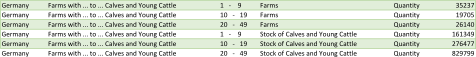
\includegraphics[width=0.5\textwidth]{images/spreadsheet_data_extractor/output.pdf}
    \caption[Output relation]{Output relation, Source: Own figure}
    \label{fig:spreadsheet_data_extractor_output}
\end{figure*}%


\subsection{Serialisation}

Ich habe eine softare entwickelt, die es ermöglicht, Daten aus Excel-Tabellen zu extrahieren. 

%\begin{verbatim}
%abstract class TaskList implements Built<TaskList, TaskListBuilder> {
%  BuiltList<ImportExcelFilesTask> get childTasks;
%
%  TaskList._();
%  factory TaskList([void Function(TaskListBuilder) updates]) = _$TaskList;
%
%  static Serializer<TaskList> get serializer => _$taskListSerializer;
%}
%\end{verbatim}

 
 


\subsection{Inkrementelles laden der Excel Dateien. }



Wenn excel Dateien öffnet, dann lädt es zunächst die gesamte Datei mit allen Arbeitsblättern, bevor das erste Arbeitsblatt zur Darstellung gebracht wird.Bei Dateien, die sehr große Arbeitsblätter enthalten, kann dies einige Sekunden bis Minuten dauern.Den Benutzer, das extrahieren aus einer.Anzahl von Excel Dateien zu erleichtern, implementierten Via einen Mechanismus zum Inkrementellen Laden von.Excel Dateien.


Eine exe Datei ist ein zip Archiv, welches einer Reihe an XML Dateien enthält, die die.Workshits die Formatierungen und wiederkehrende Texte beschreiben.Unsere Lösung öffnet zunächst das Archiv, extrahiert aber zunächst keine darin enthaltenen Dateien.Extrahiert unsere Lösung lediglich die Liste der Dateien.Dabei werden alle worksheet Dateien in dem XL worksheets Ordner Zu einem Dictionary hinzugefügt.Dieses Dictionary enthält die Informationen wie den Arbeitsblattnamen.Diese können den Benutzer, wenn er die Oberfläche zum Selektieren von Arbeitsblättern öffnet, direkt als Reiter angezeigt werden. Diese Ansicht, welcher aller Arbeitsblätter als Reiter visualisiert, kann sehr schnell den Benutzer nahezu sofort präsentiert werden, da das Öffnen der Archiv Datei sehr flott vonstatten geht.

Erst wenn der Benutzer auf einen der Reiter der Arbeitsblätter klickt.Parst  unsere Lösung Den Dateiinhalt dieses Arbeitsblattes. Sobald der Dateiinhalt dieses Arbeitsblattes komplett gelesen ist, ersetzen wir in dem Dictionary die. Den Verweis auf die Datei mit dem tatsächlichen Inhalt der Datei. Auf diese Weise wird verhindert, dass die Datei immer wieder beim Aufrufen dieses Arbeitsblattes erneut geparst wird.

Öffnet der Benutzer ein anderes Arbeitsblatt, so wird auch dieses erst beim Zugriff auf das Arbeitsblatt gepasst.Gehensweise ermöglicht es uns jeder.Excel Datei nahezu sofort dem Benutzer zur Anzeige zu bringen und ihm keine Wartezeiten im Öffnen der.Excel Dateien zuzumuten.

\subsection{Darstellung der.Arbeitsblätter}



Damit der Benutzer keine Schwierigkeiten hat, sich im Arbeitsplatz zurechtzufinden, legen wir wert darauf, die Arbeitsblätter so anzuzeigen, wie sie auch in Excel angezeigt werden.

Anzeige der Höhe und Breite

Unsere Lösung extrahiert die Informationen über die Spaltenbreiten und Zeilenhöhen aus dem Arbeitsblatt. Dabei ist darauf zu achten, dass in Excel die Spaltenbreiten und Zeilenhöhen in Excel Einheiten gemessen werden. Diese müssen mit einem Faktor mit impliziert werden, um die tatsächliche Höhe oder Breite in Pixeln zu erhalten.Wichtig dabei zu betrachten ist, dass dieser Faktor unterschiedlich ist. Für die Breite und für die Höhe.Damit die Spaltenbreite genauso bereit erscheint, wie sie in Excel erscheint, muss die angegebene Einheit in der XML Datei mit dem Faktor x multipliziert werden.Um die tatsächliche Zeilenhöher in Pixeln zu erreichen, muss dagegen der Faktor y mit dem Wert der in der exe Datei angegeben wird, multipliziert werden.

\subsection{Overflow}



Genau wie in Excel auch achten wir darauf, dass Text.Bitte die nicht in die Zelle hineinpassen.Durch einen Overflow in die anliegenden Zellen hineinragen.Doch das darf nur geschehen, wenn die anliegenden Zellen nicht selbst Werte enthalten.

Zeichnen wir die Zellen auf diese Art und Weise, erhalten wir eine Darstellung, die Excel sehr nahe kommt.

\subsection{Performance}


Sobald alle Spaltenbreiten und Zeilen Höhen extrahiert wurden, können wir diese Nutzen Um zu berechnen, welche Zellen aktuell sichtbar sind und alle anderen Zellen beim Zeichnen zu ignorieren. Dazu wird das aktuelle Scroll Offset in der x und y Achse berücksichtigt und Dabei wird berechnet.Welche Zellen aktuell sichtbar sind Indem die Spaltenbreiten so lange addiert werden, bis  die Summe die linke Kante des Viewports erreicht. Alle Zellen links davon werden beim Zeichnen ignoriert. Weiterhin werden die Spaltenbreite Breiten weiter addiert, bis sie die rechte Kante des Viewports erreicht.Alles Zellen rechts davon werden beim Zeichnen ignoriert. Weiterhin werden die Zeilenhöhen entweder aus der Standard Höhe.Des Arbeitsblattes oder über die Benutzer definierten Höhen der Zeilen extrahiert und so lange aufaddiert, bis die Summe die obere Kante des Viewports erreicht.Alle Zellen, die oberhalb dieser Kante liegen, werden beim Zeichnen ignoriert.Die Zeilenhöhen werden weiter aufaddiert, bis sie die.Unsere Kante des Viewports erreicht.Nur diese Zellen werden gezeichnet. Alle Zellen unterhalb dieser Kante werden ignoriert.




The amount of unsued cells is likely to be higher,
because our script does not check for cells that seem like they contain contentbecause they reference a shared structuring
but in reality those shared strings are just whitespaces that got into the cells by accident.
Those cells are not filter our by our script because of the performance.
Our script filters out the cells that don't have childdren with a xpath query
which is very fast in comparison to iterating
over every node and checking if the referenced shared string consists of only white spaces.

https://ecma-international.org/publications-and-standards/standards/ecma-376/

Dataset: \cite{vos2024calculations}



\section{Evaluation}


After building the first version of the Spreadsheet Data Extractor,
student assistants successfully used it to extract data from over 500 Excel files.
The time taken for each file was determined from a sample of 331 processed Excel files,
comprising 3,093 worksheets, with outliers caused by pauses removed. On average,
the student assistants required 15 minutes per file and 95 seconds per worksheet. 

Research Question 1 can be answered positively.
Student assistants without programming experience were able to extract data from over 500 Excel files
using the Spreadsheet Data Extractor in a reasonable amount of time.

\section{Outlook}

\section{Fintergrundfarben, Borders}

Um dem Benutzer das Zurechtfinden in den ziArbeitsblättern weiter zu erleichtern, könnte der Spread Sheet Data Extractor weiter erweitert werden, sodass er auch hintergrundfarben, Vordergrundfarben der Texte und Borders.Was von den Zellen genauso anzeigt, wie es auch Exi tut.



The extraction of data from the heterogeneous spreadsheet files was possible,
even though the user experience was not optimal.
Many aspects of the user experience that would have been significant time-saving features
had to be omitted during development due to time restrictions.
These included features for describing the hierarchy of the worksheets and exporting the extracted data.


\subsection{Improvements for Describing the Spreadsheet Hierarchy}

The current version of the Spreadsheet Data Extractor hampers the user experience:
\begin{itemize}
    \item The user needs to switch back and forth between the task view (Figure \ref{fig:spreadsheet_data_extractor_task_view}) and the cell selection view (Figure \ref{fig:spreadsheet_data_extractor_cell_selection_view}).
    \item To duplicate and move a hierarchy, the user must first select each node that should not be moved individually and then freeze them in place.
    \item The user needs to know in advance when to create empty nodes if the number of column headers varies from column to column.
\end{itemize}

\begin{figure}[ht]
  \centering

  \includegraphics[width=0.5\textwidth]{images/spreadsheet_data_extractor/views/task_view.png}

  \caption[The task view listing all nodes in the hiarachy graph]{The task view Listing all nodes in the hiarachy graph, Source: Own figure}
  
  \label{fig:spreadsheet_data_extractor_task_view}
\end{figure}%

\begin{figure}[ht]
  \centering

  \includegraphics[width=0.5\textwidth]{images/spreadsheet_data_extractor/views/cell_selection_view.png}

  \caption[The cell selection view]{The cell selection view, Source: Own figure}
  
  \label{fig:spreadsheet_data_extractor_cell_selection_view}
\end{figure}%

\subsubsection{Switch Between Task View and Cell Selection View}
When creating a new node to describe the task of extracting a cell or set of cells,
the user must switch to the view that displays all tasks.
To export a cell or set of cells, the user must first switch to the view that displays
the cells and then select the desired cell(s) upon node creation.
As the hierarchy of the spreadsheet grows, switching back and forth and finding
the correct nodes becomes increasingly time-consuming.

\subsubsection{Select Each Node Individually to Lock in Place}

The switching of views is increasingly complicated for the user
when duplicating and moving a hierarchy of export tasks.
While in the view showing the cells,
the user might try to duplicate a hierarchy by extracting one sub-table
of a sheet and then move that hierarchy to the next sub-table below.
Only at that point, the user might see that the table below does not repeat the column headers,
and the user might want to freeze those nodes in place.

To freeze the nodes the user needs to switch to the task view once again.
There, they need to look up all nodes that represent the column headers.
The user can only identify those nodes by their extracted value and their cell coordinate,
while it would be much easier to just see the centre in the actual grid.
The column headers are scattered across the whole hierarchy,
which means it will take the user a while to scroll through the hierarchy,
reminding themselves of the extracted values from those column headers
and comparing them with the values shown in the task list.

After the user has used the freeze function,
they can switch back to the view showing the worksheet cells and repeat
the step of duplicating and moving the hierarchy.
Only by that time will the user see if they correctly froze the correct nodes
or if they missed nodes or even selected the wrong ones.

\subsubsection{The User Needs to Know Beforehand When to Create Empty Nodes}



Many tables in our dataset have columns with varying count of headers.
For instance, in Figure \ref{fig:sheeps_columns}
\cite{SB23},
there is one column with the header \textit{Total}
and another with the headers \textit{Ewes}, \textit{Dairy Sheep}, and \textit{Namely}.
The header \textit{Namely} is unnecessary, but \textit{Ewes} is valuable metadata
and should be included in the output relation.
To preserve all metadata, there are two possible solutions.
Columns with multiple headers could be concatenated with a delimiter,
such as \textit{Ewes-Dairy Sheep}.
This would ensure that the number of headers in the column is consistent.
However, this solution has the disadvantage of losing the hierarchy of the headers,
making it impossible to filter the resulting dataset for the metadata \textit{Ewes}.
The second solution would be to add empty nodes for the columns with fewer headers
to match the count of headers in all columns.
In this example, \textit{Total} and \textit{Dairy Sheep} can be treated as metadata of the same level.

\begin{figure*}[t]
    \centering
    \includegraphics[width=\textwidth]{images/spreadsheet_data_extractor/sheeps_columns.pdf}
    \caption[Varying count of column headers]{Varying count of column headers, Source: Own figure}
    \label{fig:sheeps_columns}
\end{figure*}%

Adding an empty node with the child \textit{Total}
results in the output relation for the rows \textit{Total} and \textit{Dairy Sheep},
as shown in Figure \ref{fig:sheeps_columns_output}.

\begin{figure}[t]
    \centering
    \includegraphics[width=\linewidth]{images/spreadsheet_data_extractor/sheeps_columns_output.pdf}
    \caption[Output relation with empty nodes]{Output relation with empty nodes, Source: Own figure}
    \label{fig:sheeps_columns_output}
\end{figure}%


To accomplish this, the user must be aware
at the moment they select the \textit{Total} column,
that subsequent columns will have additional column headers.
Therefore, they need to preemptively create an empty node
as the parent of the \textit{Total} node.
If the user forgets to create this parent node
and only realizes the discrepancy in the number of column headers
in subsequent columns, they currently have
to tediously modify the hierarchies of the previous columns.
The user can initially copy the \textit{Total} node,
then delete it, add an empty node in its place,
and finally insert the copied \textit{Total} node as its child.
This process involves a significant number of steps for the user,
resulting in a poor user experience.




 
Improving the user experience of this application could be achieved through several enhancements:

\subsubsection{Integration of Task and Cell Selection Views}

The hierarchy of cell selections could be shown as a side panel, or even better as graphs in the view showing the cells.
In the current version of the Spreadsheet Data Extractor the selected cells are already highlighted.
The hierarchy could be shown by connecting the highlighted sets of cells with arrows pointing to their parent and child nodes.

\subsubsection{Support for Multi-Node Selection}
If the user wishes to freeze cells before duplicating and moving a hierarchy,
the user should be able to select these cells by clicking directly on them.
This could be sped up by allowing the user to select multiple sets of cells
by drawing a line around them,
as is done in other GUIs and is often referred to as the lasso tool.

\subsubsection{Drag-and-Drop Node Manipulation}
Enabling users to drag and drop nodes to rearrange them
within the hierarchy would simplify the process
of organizing and structuring data,
providing a more intuitive way to describe the hierarchy and 
allowing for quick corrections in case of errors.

\subsubsection{Node Wrapping Functionality}

Introducing the feature to wrap user-selected nodes
into new ones would provide users with the flexibility
to create empty nodes on-the-fly as they recognize the need for them.
For example, if a user adds a new column
with more column headers than the existing ones,
they could seamlessly wrap the previous column headers into new nodes
to match the number of headers in each column. 

\subsection{Enhancements for Data Export}


While the extraction of the more than 500 Excel files was a success, it resulted in a few hundred CSV files.
All of these files are in a machine-readable format but are split into many separate files.
A lot of those files have the same amount columns and the  same or a very similar set of metadata columns.
Those files should be combined, because they contain the same type of data, yet different values.
The reason for this is, because the Spreadsheet Data Extractor made it easy for the user to extract data from just one or a few of Excel files.
Using it for a lot of files was impractical, because the task view grew very big with just extracting from one file.
To maintain an overview the student assistants instead created a new configuration when moving to the next Excel file.
That means that the extracted files needed to be combined afterward by comparing them with each other.
When two files are similar, they needed to be merged into a single file


To streamline this process the user experience could be improved by implementing an
input- and output-manager.

\subsubsection{Input Manager}

Firstly, an Input Manager within the Spreadsheet Data Extractor
should facilitate the import of all files,
offering users a comprehensive overview
of all imported files directly within the application.
This feature would discourage users from organizing files externally
and ensure centralized management of file imports.

Additionally, the Input Manager should indicate the extent to which each file's data
has been described through cell selections.
This would aid users in finding out which files need to be processed next 
and prevent the need for manual organization of files into directories called "to-do" and "done".


\subsubsection{Output Manager}

Secondly, the Spreadsheet Data Extractor requires an Output Manager.
Instead of exporting hierarchies directly to CSV files,
users should first define a target format specifying column names, data types, and desired order.
Subsequently, users can progressively link newly described hierarchies to existing output formats.
This facilitates efficient data consolidation.
Once all files are described and linked, data can be exported as a small set of CSV files,
ensuring consistency and ease of use.

\bibliographystyle{ACM-Reference-Format}
\bibliography{sample-base}


\end{document}
\endinput
